Nachdem die theoretischen Grundlagen und der Aufbau des ALICE Experiment n\"aher erl\"autert wurden, wird im folgenden die Vorgehensweise erkl\"art, wie $\pi^{0}$ gemessen werden.
\newline
Die in Abschnitt \ref{s3s1s2} genannten Auswahlkriterien von \textit{Clustern}, filtern die \textit{Cluster} so, dass haupts\"achlich \textit{Cluster} die aus einen Photon, Elektron oder Positron entstanden, \"ubrig bleiben.
\newline
\begin{figure}[thp]
\centering
\includegraphics[width=.7\linewidth]{hInvMass_pT_Signal.pdf}
\caption{$p_\text{T}$ und $m_\text{inv}$ als Funktion von der Anzahl von rekombinierten  Cluster-Paaren aus der gleichen Kollision.
Die rote Linie liegt bei $m_{\text{inv}}\approx,135\rm{GeV/}c^{2}$, was in etwa der $\pi^{0}$ Masse entspricht, wo eine deutliche H\"aufung der Eintr\"age sich abzeichnet.
Die schwarzen Linien stellen die Grenzen der $p_{\rm{T}}$-Intervalle dar.}
\label{figInvMassPt_a}
\end{figure}
Um $\pi^{0}$ messen zu k\"onnen, werden aus den Photonenkandidaten, die zu den genannten \textit{Clustern} korrespondieren, die invariante Masse und der Transversalimpuls nach Gleichungen \ref{eq_invmass} und \ref{eq_pt} bestimmt.
Da die Information, ob und welche Photonenkandidaten von einem $\pi^{0}$ stammen, fehlt, werden alle Photonenkandidaten eines \textit{Events} mit einander kombiniert.
Dieses Vorgehen wird als \textit{same event method} bezeichnet.
Abbildung \ref{figInvMassPt_a} zeigt die Anzahl solcher Rekombinationen in abh\"angigkeit der invarianten Masse $m_{\rm{inv}}$ und des Transversalimpulses $p_{\rm{T}}$.
Durch die Kombination aller Photonenkandidaten eines \textit{Events} gibt es sowohl Rekombinationen zusammengeh\"origer Photonenkandidaten, als auch unabh\"angiger Photonenkandidaten.
Es zeichnet sich eine Anh\"aufung der Datenpunkte um $m_{\rm{inv}}\approx 0,135\rm{GeV}/c^{2}$, also um die Masse von $\pi^{0}$, ab.
Dieser Anh\"aufung liegen vor allem Rekombinationen zusammengeh\"origer Photonenkandidaten zugrunde.
Die Form der linken Kante liegt dem \textit{opening angle cut} zugrunde.
\newline
Die $p_{\rm{T}}$-Ab\"ahngigkeit der Anzahl der $\pi^{0}$ weist auf unterschiedliche physikalische Effekte und Prozesse hin.
Deshalb wird die Verteilung aus Abbildung \ref{figInvMassPt_a} integriert \"uber einzelne $p_{\rm{T}}$-Intervall betrachtet und analysiert.
Die Intervalle werden so gew{\"a}hlt, dass sie m{\"o}glichst klein sind, w{\"a}hrend die statistischen Unsicherheiten nicht zu gro{\ss} werden.
\begin{figure}[tbp]
\centering
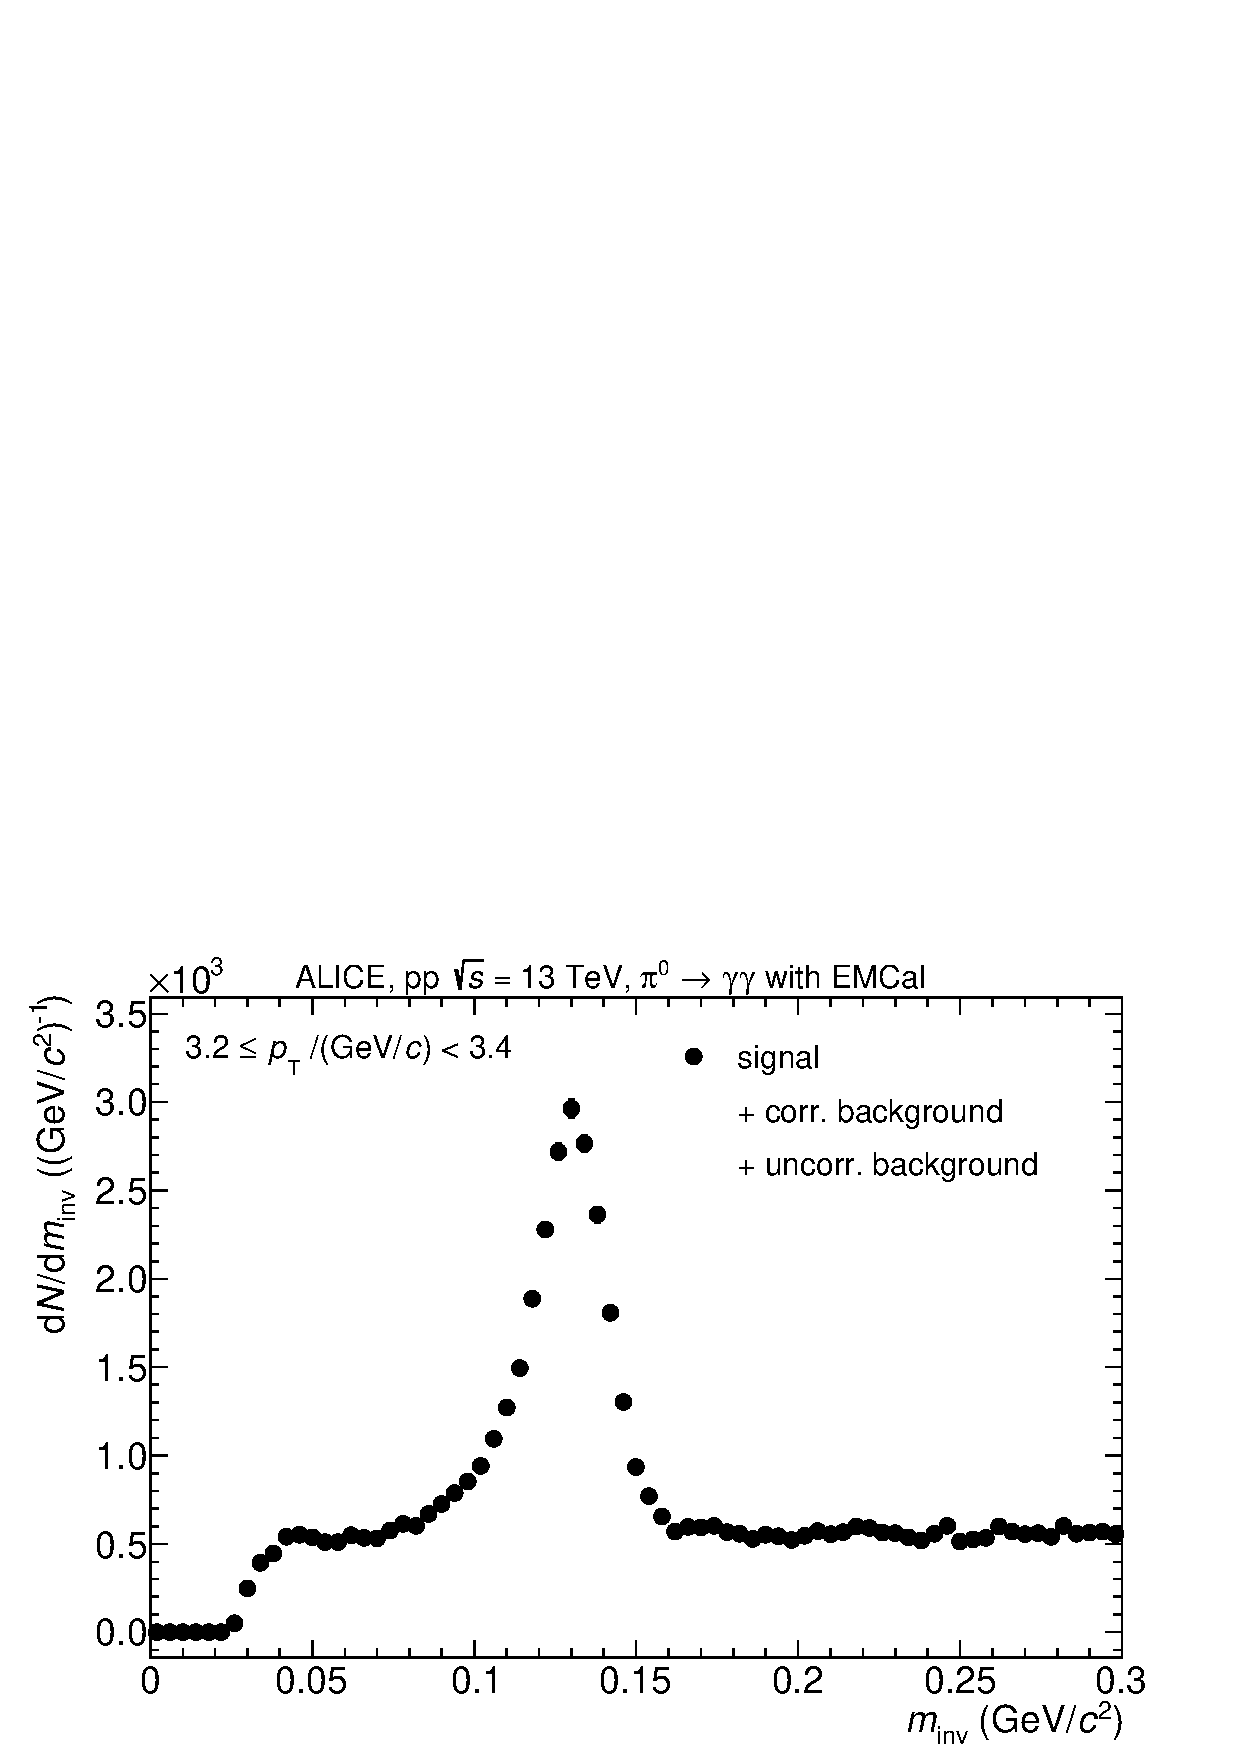
\includegraphics[width=.75\linewidth]{hSignalPlusBkg.pdf}
\caption{Projektion von Abbildung \ref{figInvMassPt_a} im $p_{\text{T}}$-Intervall $(3,2 - 3,4) (\text{GeV/}c)$. Es ist ein deutlicher Peak um $m_{\pi^{0}} \approx 0,135\text{GeV/}c^{2}$ zu erkennen, aber auch Untergrund, da das Signal zu h{\"o}heren Massen gau{\ss}f{\"o}rmig abklingen sollte. Bei $m_{\text{inv}} < m_{\pi^{0}}$ kann Signal vorliegen, das aus konvertierten Photonen besteht, weshalb eine Aussage {\"u}ber die Form, bzw. den Untergrund dort schwer m{\"o}glich ist.}
\label{figSignalPlusBkg}
\end{figure}
\newline
Abbildung \ref{figSignalPlusBkg} zeigt eine invariante Massenverteilung in einem $p_{\text{T}}$-Intervall von $(3,2 - 3,4)(\rm{GeV/}c)$.
Die zuvor beschriebene Anh\"aufung von Datenpunkten in Abbildung \ref{figInvMassPt_a} zeigt sich auch hier deutlich und wird im folgenden als \textit{Peak} bezeichnet.
Der Peak besteht wie oben erw\"ahnt hauts\"achlich aus richtig rekombinierten $\pi^{0}$.
Die Summe aller richtig rekombinierter $\pi^{0}$ wird als Signal bezeichnet.
Neben dem Signal besteht die Verteilung in Abbildung \ref{figSignalPlusBkg} noch aus sogenanntem Untergrund, der in zwei Teile unterteilt wird, den kombinatorischen oder auch unkorrelierten Untergrund und der korrelierte Untergrund.
Durch die Kombination unkorrelierter Photonenkandidaten, also solcher, die \"uber keinen Zerfall zusammenh\"ahngen, entsteht der unkorrelierte Untergrund.
Dem korrelierte Untergrund hingegen liegen Kombinationen von Photonenkandidaten zugrunde, zwischen denen, wieder Name andeutet, einen Korrelation besteht.
\newline
Im folgenden Abschnitt wird eine Methode zur Absch\"atzung des unkorrelierten Untergrunds vorgestellt und durchgef\"uhrt. 